\chapter{Elettrodinamica}

Andremo in questo capitolo ad introduttore il \textbf{tempo} in tutta la trattazione vista fino a questo punto. 

\section{Conduzione Elettrica}
Ricordiamo che le equazioni di Maxwell in elettrostatica valgolo solamente, come suggerisce il nome, in condizioni di $t = 0$. In questo capitolo, questa ipotesi viene abbattuta, dunque avremo la necessità di andare a rivedere tali equazioni al fine di adattarle al nuovo contesto in cui ci troviamo. 

In particolare, dato che per fare scorrere una carica in un circuito è necessario compiere lavoro, la seconda equazione andrà rivista..

Avendo delle cariche in moto, su tali cariche agirà una forza $F = qE$ e dunque il lavoro $L = \oint F ds = ... q\oint E \ne 0$. In sostanza il \textbf{campo elettrico non è conservativo} e quindi \textit{serve del lavoro per mantenere le cariche in moto}. 

\subsection{Corrente Elettrica e Forza Elettromotrice}
Ipotizziamo di avere due conduttori, uno di questi a $V^+$, l'altro $V^-$, collegati con un filo di rame che non contribuisca al nostro sistema. Sappiamo che dal potenziale maggiore al potenziale minore avremo un campo elettrostatico. 

\begin{figure}[H]
	\centering
	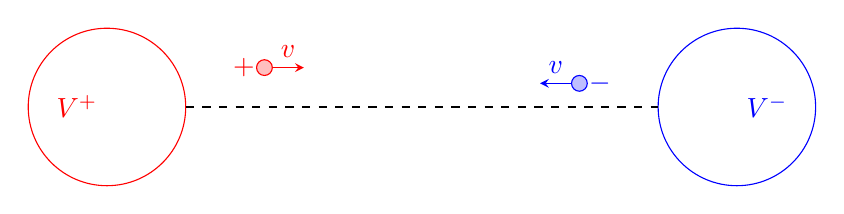
\begin{tikzpicture}
		\draw[color = red] (-4, 0) circle [radius = 1] node [left] {$V^+$};
		\draw[color = blue] (4, 0) circle [radius = 1] node [right] {$V^-$};
		
		\draw [dashed] (-3,0) -- (3,0);
		
		\draw [color=red, fill=red!25] (-2,0.5) circle [radius=0.1] node [left] {$+$};
		\draw [color=blue, fill=blue!25] (2,0.3) circle [radius=0.1] node [right] {$-$};
		
		\draw [color=red, -stealth] (-1.9,0.5) -- (-1.5, 0.5) node [midway, above] {$v$};
		\draw [color=blue, -stealth] (1.9,0.3) -- (1.5, 0.3) node [midway, above] {$v$};
		\end{tikzpicture}
\label{fig:corrente}
\caption{Corrente}
\end{figure}

Vediamo come, una volta collegati i due conduttori, inizia un \textbf{moto di cariche} che terminerà nel momento in cui i due conduttori avranno raggiunto lo stesso potenziale. Per mantenere le cariche in moto abbiamo bisogno di ripristinare continuamente la differenza di potenziale. Per fare questo avrò bisogno di un nuovo oggetto che agisca nella direzione opposta rispetto al campo: un \textbf{generatore}. La forza che sposta nuovamente le cariche positive in modo da ripristinare il potenziale, è detta \textbf{forza elettromotrice}. 

\begin{large}
	\begin{equation} \label{eq_fem}
		f.e.m. \;\; \mathcal{E} = \int_A^B \frac{F}{q} dl = V^+_B - V^-_A
	\end{equation}
\end{large}

tale $f.e.m.$ è detta anche \textbf{tensione} o \textbf{differenza di potenziale} $ddp$.

\begin{figure}[ht]
	\centering
	\begin{tikzpicture}
		\draw (0,0) -- (0,3) -- (4,3) -- (4,0) -- (2.5,0) (0,0) -- (1.5,0);
		\draw (2.5, 0.5) -- (2.5, -0.5) (1.5, 0.7) -- (1.5, -0.7);
		
		\node at (2.75, -0.7) {$-$};
		\node at (1.25, -0.7) {$+$};
		
		\draw [-stealth] (-0.5, 1) -- (-0.5, 2) node [midway, left] {$E$};
		\draw [-stealth] (1,3.3) -- (3, 3.3) node [midway, above] {$E$};
		\draw [-stealth] (4.5,2) -- (4.5, 1) node [midway, right] {$E$};
		\draw [-stealth] (1.7, 0.4) -- (2.3, 0.4) node [midway, above] {$E$};
		\draw [color=red, -stealth] (2.3, -0.4) -- (1.7, -0.4) node [midway, below] {$E*$};
	\end{tikzpicture}
\end{figure}

Considerando la situazione seguente, andiamo a calcolare la circuitazione, otteniamo che 

$$
\oint E_{elettrostatico} + E^* \ne 0
$$

Il risultato dell'integrale di cui sopra è proprio la forza elettromotrice. Definiamo quindi nel seguente modo la \textbf{forza elettromotrice}: 

\begin{large}
	\begin{equation}
		\mathcal{E} = \oint E^* \;\; \left[V\right]
	\end{equation}
\end{large}

\subsection{Intensità di Corrente}
Definiamo \textbf{intensità di corrente} $i$ la quantità di carica che scorre nell'unità di tempo attraverso una \textbf{certa superficie}. Tale valore è una quantità scalare, il cui segno va a rappresentare il verso di scorrimento delle cariche. Per convenzione si considera positiva l'intensità legata al moto di cariche positive, e negativa quella legata al moto di cariche negative:

\begin{large}
	\begin{equation} \label{eq_intensita_corrente}
		i\coloneqq \frac{dq}{dt} \;\; \left[A\right]
	\end{equation}
\end{large}

Per chiarire meglio il concetto di "attraverso una cerca superficie" abbiamo bisogno del concetto di \textbf{densità di corrente} $\vec{j} $, ovvero la quantità di carica che passa attraverso la superficie unitaria orientata in modo ortogonale al moto della carica, in pratica l'intensità non è altro che il \textbf{flusso} tramite tale superficie: 

\begin{large}
	\begin{equation}
		i = \int_{sup} \vec{j} \cdot d\vec{S}
	\end{equation}
\end{large}

dove $\vec{j}$ è la densità di corrente, che si misura in $\left[\frac{A}{m^2}\right]$. Da punto di vista microscopico ci troveremo nella situazione seguente: 

\begin{figure}[ht]
	\centering
	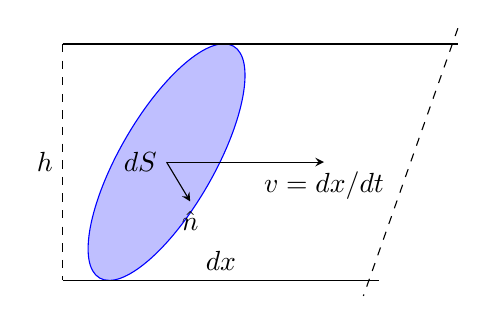
\begin{tikzpicture}
		\draw[rotate=150, color=blue, fill=blue!25] (0,0) ellipse (0.6 and 1.7) node [color=black, left] {$dS$};
		\draw (-1.32, 1.5) -- (3.7,1.5);
		\draw (-1.32, -1.5) -- (2.7,-1.5) node [midway, above] {$dx$};
		\draw[-stealth] (0,0) -- (2,0) node [below] {$v = dx/dt$};
		\draw[-stealth] (0,0) -- (0.3, -0.5) node [below] {$\hat{n}$};
		
		\draw [dashed] (3.7, 1.7) -- (2.5, -1.7);
		\draw [dashed] (-1.32, 1.5) -- (-1.32, -1.5) node [midway, left] {$h$}; 
		
	\end{tikzpicture}
\end{figure}

Abbiamo che l'intensità di corrente $i$ è data dalla carica $q$ nel cilindretto di lato $v dt$, aprendo tale formula otteniamo che l'intensità è data da: 

\begin{large}
	\begin{equation}
		i = Nq_evdS \cdot \hat{n}
	\end{equation}
\end{large}

In questa formula avremo che $N$ rappresenta il numero di elettroni per unità di volume, ciò moltiplicato per $q_e$ va a fornirci la carica totale che scorre all'interno del volumetto. La formula $dS \cdot \hat{n}$ ci permette di trovare il valore di $h$. 

Siccome $i $ è il flusso della densità di corrente $j$, abbiamo trovato la formula della \textbf{densità di corrente a livello microscopico}: 

\begin{large}
	\begin{equation}
		\vec{j} = Nq\vec{v}
	\end{equation}
\end{large}

\subsection{Corrente Stazionaria}
Parliamo di \textbf{corrente stazionaria} o \textbf{continua} quando abbiamo a che fare con una corrente in cui l'intensità $i$ nella sezione del conduttore è \textbf{costante}.  Questo chiaramente non implica il fatto che la sezione del conduttore rimanga costante, dunque nel momento in cui il conduttore ha una sezione variabile, varierà di conseguenza la \textbf{densità di corrente}.

\begin{figure}[ht]
	\centering
	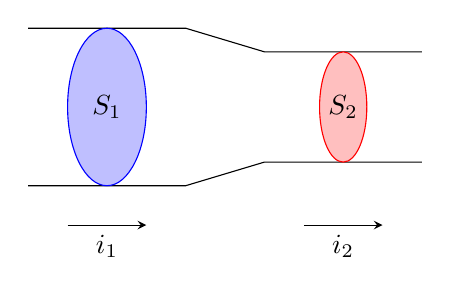
\begin{tikzpicture}
		\draw (0,2) -- (2,2) -- (3,1.7) -- (5,1.7);
		\draw (0,0) -- (2,0) -- (3,0.3) -- (5,0.3);
		
		\draw[color=blue, fill=blue!25] (1,1) ellipse (0.5 and 1) node [color=black] {$S_1$};
		\draw[color=red, fill=red!25] (4,1) ellipse (0.3 and 0.7) node [color=black] {$S_2$};
		
		\draw [-stealth] (0.5,-0.5) -- (1.5, -0.5) node [midway, below] {$i_1$};
		\draw [-stealth] (3.5,-0.5) -- (4.5, -0.5) node [midway, below] {$i_2$};
	\end{tikzpicture}
	\caption{Corrente Stazionaria}
\end{figure}

Chiaramente per mantenere l'uguaglianza tra $i_1$ e $i_2$ è necessario che valga la relazione $j_1 	\ll j_2$, soltanto in questo modo ci sarà possibile scrivere $j_1S_1 = j_2S_2$.

\section{Legge di Ohm}
Andiamo a vedere la fenomenologia microscopica alla base di questa importante legge della fisica. Ipotizziamo infatti di fare uno zoom su un conduttore che va a collegare i capi di un generatore, che va quindi a formare un circuito. All'interno di tale conduttore, a \textit{causa della temperatura} abbiamo delle cariche in moto libero disordinato (la media di tale moto è chiaramente nulla). Nel momento in cui accendiamo un campo, tali cariche iniziano un moto ordinato contro le collisioni dovute all'agitazione termica. 

In sostanza avremo che la velocità media $\left< \vec{v}_{termica}\right> = 0$ e che la media della velocità di deriva $\left< \vec{v}_{deriva} \right> \ne 0$. Avremo dunque che la densità $j = Nq\left< v_{deriva} \right>$. Mentre la velocità termica ha un ordine di grandezza di $10^2 m/s$, mentre la velocità di deriva è dell'ordine di grandezza di $10^{-5} m/s$.

\medskip

Possiamo osservare in modo sperimentale che la differenza di potenziale ai capi di un conduttore è proporzionale all'intensità, il fattore di proporzionalità è una caratteristica intrinseca del conduttore in questione. 

\begin{tcolorbox}[colframe=red, colback=red!10, title=Legge di Ohm]
	\begin{large}
		\begin{equation}
			V = Ri
		\end{equation}
	\end{large}
\end{tcolorbox}

Tutti i conduttori che rispettano questa legge sono detti \textbf{conduttori ohmici}. La resistenza si esprime in $\Omega$ e dipende dal materiale di cui un conduttore si compone oltre che dalla sua geometria, in particolare avremo quindi che 

\begin{large}
	\begin{equation}
		R = \rho \frac{l}{S}
	\end{equation}
\end{large}

Il  valore $\rho$ è detto \textbf{resistività del materiale}, per quanto riguarda invece la geometria del conduttore, avremo quindi che la resistenza aumenta con la lunghezza del conduttore e che è inversamente proporzionale alla sezione del conduttore. 

\subsection{Legge di Ohm Locale}

Dopo aver visto ciò che accade macroscopicamente, facciamo uno zoom internamente al conduttore preso in considerazione e andiamo a vedere cosa succede a livello microscopico: 

\begin{figure} [ht]
	\centering
	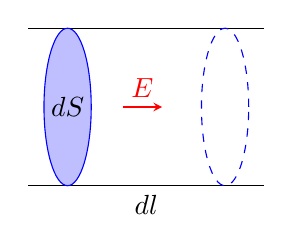
\begin{tikzpicture}
		\draw (0,1) --(3,1) (0,-1) -- (3,-1) node [midway, below] {$dl$}; 
		\draw[color=blue, fill=blue!25] (0.5, 0) ellipse (0.3 and 1) node [color=black] {$dS$};
		\draw[dashed, color=blue] (2.5,0) ellipse (0.3 and 1);
		
		\draw [-stealth, color=red] (1.2, 0) -- (1.7, 0) node [midway, above] {$E$};
	\end{tikzpicture}
\end{figure}

Applicando in questa situazione la legge di Ohm abbiamo che

$$
dV = Rdi
$$ 

e, inserendo quanto conosciamo già sull'intensità di corrente: 

$$
\begin{cases}
	di = jdS \\
	dV = Edl
\end{cases}
$$

Sostituendo opportunamente le due identità di cui sopra, otteniamo di seguito la formula, che una volta semplificata ci darà la legge di ohm valida in ambito microscopico: 

\begin{large} 
\begin{equation}
	Edl = \rho \frac{dl}{dS} j dS 
\end{equation}
\end{large}

\begin{tcolorbox}[colframe=red, colback=red!10, title=Legge di Ohm Locale]
	\begin{large}
		\begin{equation}
				\vec{E} = \rho \vec{j}
		\end{equation}
	\end{large}
\end{tcolorbox}

Cercando di ottenere il valore di $\vec{j}$ abbiamo $j = \sigma E$, il valore $\sigma = 1/\rho$ è detto \textbf{conducibilità elettrica}. 

\section{Potenza Elettrica - Effetto Joule}
Sia una resistenza attraverso la quale sta scorrendo una intensità di corrente, dunque presentemente un insieme di cariche. Sappiamo che il moto di queste cariche è reso possibile grazie ad un lavoro esterno, calcolabile tramite $dL = Vdq$ fornito dal \textit{generatore}. Nel momento in cui abbiamo un lavoro, possiamo anche trovare la \textbf{potenza} data dal lavoro per unità di tempo $P = dL/dt$: 

\begin{equation} \label{eq_potenza_elettrica}
	P_{elettrica} = V\frac{dq}{dt} \; = \; Vi \; \; [W]
\end{equation}

Questa è in pratica la \textbf{potenza elettrica erogata} dal generatore per avere l'intensità $i$. Se dovesse anche valere la legge di Ohm, avremo anche che 

\begin{equation}
	P = Ri^2 = \frac{V^2}{R}
\end{equation}

Questa equazione ci dà invece l'espressione della \textbf{potenza dissipata} nel \textbf{materiale}; tale dissipazione è anche detta \textbf{effetto Joule}, l'effetto ultimo è quello della produzione di \textit{calore}.

Potremmo essere interessati a raccogliere la potenza erogata $Vi$ in un \textbf{capacitore}. Andremo successivamente a sviluppare questa trattazione.

\subsection{Bilancio Energetico di un Circuito}
Supponiamo di essere sempre in corrente stazionaria, di avere un circuito dotato di un generatore $\mathcal{E}$ e di una certa resistenza $R$. Abbiamo che la potenza generata $P_{gen} = \mathcal{E}i$, e che la potenza dissipata $P_r = Ri^2 = Vi$, dove $V$ è la differenza di potenziale ai capi di $R$. In questo modo, stiamo dicendo che la potenza viene \textbf{dissipata lungo tutto il circuito}. 

$$
L = \int_{tempo} Pdt  \; \; \longrightarrow \;\; L_{tot gen.} = \mathcal{E}_i \Delta t = L_{dissipato R} = Ri^2 \Delta t
$$

Chiaramente, nel caso in cui abbiamo all'interno del nostro circuito anche un condensatore avremo che $L_{tot} = L_{dissipato} + L_{en.immagazzinata}$


\paragraph{Osservazione} Considerando un'altra formulazione della potenza, sappiamo che $P = F\cdot v$ e, sostituendo $F = qE$ troviamo $P = qE \cdot V$, ma sappiamo che $qv = j$, dunque potremo anche scrivere: 

$$ P_{dissipata} = \vec{j} \cdot \vec{E} $$

Facciamo ora riferimento all'immagine seguente: 

\begin{figure}[th]
	\centering
	\includegraphics[width=0.5\linewidth]{Media/circuito_1}
	\label{fig:circuito1}
\end{figure}

In questo caso avremo che la $f.e.m.$ prodotta dal generatore, sarà quella necessaria a \textit{ristabilire le cadute di potenziale }dovute alle due resistenze nel circuito, dunque, applicando ohm avremo che: 

\begin{equation} \label{eq_bilancio_potenziale}
f.e.m. = Ri + ri 
\end{equation}

Questa equazione ci fornisce il bilancio energetico del nostro circuito in termini di \textbf{potenziale}.
Se ad esempio vogliamo trovare la differenza di potenziale ai capi della resistenza di carico, questa sarà data da $Ri$, ovvero $\mathcal{E} - ri$: in pratica togliamo alla $f.e.m$ totale tutto il potenziale fatto cadere dagli altri elementi del circuito. Un altro modo per esprimere tale valore è il seguente: 

$$V_a - V_b = Ri = \frac{\mathcal{E}}{1 + r/R} $$

In sostanza la formula di cui sopra ci dice che se vogliamo misurare la forza elettromotrice dovremo farlo a \textit{circuito aperto}, ovvero con $R \rightarrow \infty$, $i \rightarrow 0$ e dunque, la $f.e.m.$ è data dalla differenza di potenziale ai capi della resistenza di carico. 

Per trovare il bilancio energetico in termini di \textbf{energia}, aggiungiamo all'equazione della $f.e.m.$ \ref{eq_fem} la carica, sapendo che $dq = idt$: 

\begin{equation} \label{eq_bilancio_energia}
	\mathcal{E}idt = Ri^2dt + ri^2dt
\end{equation}

Dal bilancio in energia, togliendo il tempo, avremo anche il bilancio nelle \textbf{potenze}: 

\begin{equation}
	\label{eq_bilancio_potenza}
	\mathcal{E}i = Ri^2 + ri^2
\end{equation}

\section{Collegamento di Resistori}
Così come per i capacitori, anche per quanto riguarda i resistori abbiamo la possibilità di effettuare un collegamento in \textbf{serie} o in \textbf{parallelo}. 

\paragraph{Collegamento in Serie}
Definiamo questo tipo di collegamento tramite il fatto che per i resistori collegati in serie passa la \textbf{stessa corrente}

\begin{figure}[th]
	\centering
	\includegraphics[width=0.5\linewidth]{Media/Resistenze_serie}
	\caption{Resistenze in Serie}
	\label{fig:resistenzeserie}
\end{figure}

In questo caso la resistenza \textit{equivalente} sarà data da: 

\begin{equation}
	\label{eq_serie}
	V{tot} = \sum^n V_i = \sum^n R_i i  = i \sum^n R_i
\end{equation}

In sostanza avremo dunque che il collegamento in serie serve ad aumentare la resistenza totale: 

$$ R_{eq} = \sum_{i=1}^n R_i $$

\paragraph{Collegamento in Parallelo}
Questo collegamento è invece caratterizzato dal fatto che ai capi delle resistenze abbiamo la \textbf{stessa differenza di potenziale}

\begin{figure}[th]
	\centering
	\includegraphics[width=0.5\linewidth]{Media/Resistenze_parallelo}
	\caption{Resistenze in Parallelo}
	\label{fig:resistenzeparallelo}
\end{figure}

In questo caso, avremo invece che la resistenza \textit{equivalente} è data da: 

\begin{equation}
	\label{eq_parallelo}
	i_{tot} = \sum^n i_i = \sum^i  \frac{V_i}{R_i} = V \sum_{i=1}^n \frac{1}{R_i}
\end{equation}

In pratica avremo che questo tipo di collegamento è utilizzato per abbassare il valore della resistenza equivalente, e dunque $$\frac{1}{R_{eq}} = \sum_{i=1}^n \frac{1}{R_i} = \frac{R_1R_2}{R_1 + R_2}$$

\paragraph{Partitore Resistivo}
Si tratta di un oggetto che ripartisce la equamente la \textbf{tensione} tra le resistenze collegate in \textbf{serie} all'interno del nostro circuito. 

\begin{figure}[th]
	\centering
	\includegraphics[width=0.5\linewidth]{Media/partitore_resistivo}
	\caption{Partitore Resistivo Serie}
	\label{fig:partitoreresistivo}
\end{figure}

Come già anticipato si tratta di un oggetto componibile tramite il collegamento in serie di $n$ resistenze collegate ad un generatore. È abbastanza immediato vederlo come un circuito elementare composto dal generatore e dalla resistenza equivalente di cui abbiamo già dato la formulazione. Avremo quindi che: 

$$
i = (i_1 = i_2) = \frac{\mathcal{E}}{R_1 + R_2} 
$$

Chiaramente questa formulazione è ottenuta utilizzando un'inversa di  \ref{eq_serie}, ricordando che la differenza di potenziale è praticamente $\mathcal{E}$. 
Si noti come l'intensità sia la stessa ai capi di $R_1$ e di $R_2$, tipica caratteristica del collegamento in serie. 


Se vogliamo invece verificare $V_1$ e $V_2$ avremo che questi sono espressi nel modo seguente: 

$$
\begin{cases}
	V_1 = R_1 i = \frac{R_1}{R_1 + R_2} \mathcal{E} \\
	V_2 = R_2 i = \frac{R_2}{R_1 + R_2} \mathcal{E}
\end{cases}
$$

Nel caso in cui le resistenze siano invece collegate in \textbf{parallelo} avremo che ad essere ripartita sarà l'\textbf{intensità di corrente}. Avremo dunque una resistenza equivalente data da $R_{eq} = \frac{R_1R_2}{R_1 + R_2}$. L'intensità di corrente ai capi delle due resistenze sarà invece: 

$$
	\begin{cases}
		i_1 = \frac{\mathcal{E}}{R_1} = \frac{R_2}{R_1 + R_2} i \\
		i_2 = \frac{\mathcal{E}}{R_2} = \frac{R_1}{R_1 + R_2} i
	\end{cases}
$$

\subsection{Potenze}
Dato che la potenza è locale, avremo che la potenza è sempre la somma delle potenze dissipate dai singoli elementi del circuito: $P_{tot} = \sum R_i i^2 = R_{eq}i_{tot}^2$. 

\begin{equation}
	P_{serie} = (R_1 + R_2) i^2_{tot}
\end{equation}

\begin{equation}
	R_{parallelo} =  R_1i_1^2 + R_2i_2^2 = \mathcal{E}^2 \left(\frac{1}{R_1} + \frac{1}{R_2}\right)
\end{equation}

\section{Leggi di Kirchhoff}
In questo punto del corso stiamo trattando le \textit{reti lineari}, nelle quali abbiamo a che fare con resistori e generatori. Una qualsiasi rete elettrica è rappresentabile utilizzando due elementi principali: 

\begin{itemize}
	\item \textbf{Nodi}: oggetti nei quali confluiscono più rami
	\item \textbf{Maglie}: caratterizzate da un verso di percorrenza della corrente 
\end{itemize}

Le leggi di Kirchhoff impongono dei vincoli sui nodi e sulle maglie: 

\begin{tcolorbox}[ title=1° Legge di Kirchhoff]
	Considerando un nodo avremo che la somma delle correnti uscenti e delle correnti entranti è sempre nulla. Per convenzione consideriamo uscenti le correnti positive, entranti quelle negative.
	\begin{large}
		\begin{equation}
			\sum_k i_k = 0
		\end{equation}
	\end{large}
\end{tcolorbox}

Si noti come tale legge è fortemente legata alla \textbf{conservazione della carica}.

\begin{tcolorbox}[ title=2° Legge di Kirchhoff]
	Associando un verso alla maglia, avremo che la somma delle tensioni (elementi passivi) in una maglia con i segni decisi dal verso assegnato alla maglia, è uguale alla somma degli elementi passivi che producono cadute di potenziale.
	\begin{large}
		\begin{equation}
			\sum_k \mathcal{E}_k = \sum_k R_k i_k
		\end{equation}
	\end{large}
\end{tcolorbox}

\section{Carica e Scarica di un Condensatore}
Torniamo ora a quanto descritto nell'immagine \ref{fig:corrente} e ipotizziamo di collegare i due conduttori in questione tramite un file di rame, che sarà dotato di una sua resistenza $R_{filo}$. Vogliamo ora andare ad indagare l'intensità di corrente e la potenza. 

\begin{figure}[th]
	\centering
	\includegraphics[width=0.5\linewidth]{Media/scarica_condensatore}
	\caption{Scarica di un Condensatore}
	\label{fig:scaricacondensatore}
\end{figure}

Possiamo riassumere la struttura descritta con il circuito di cui sopra. Nel momento in cui l'interruttore viene chiuso le cariche inizieranno a scorrere dalla lastra del condensatore a potenziale maggiore verso quella a potenziale minore.

 È chiaro come la carica che scorrerà nel circuito sarà variabile nel tempo, così come la carica immagazzinata nel condensatore, questo a motivo del fatto che il condensatore si scarica. Così come le cariche variano nel tempo, lo farà anche il potenziale, questo perché la capacità del condensatore deve rimanere costante. 
 
 Chiameremo $Q$ la carica immagazzinata nel condensatore, e $q$ quella che scorre nel circuito a causa della scarica del condensatore. 
Nel momento in cui a $t_0$ viene chiuso l'interruttore abbiamo $Q(t_0) = Q_0$. 

$$ \begin{cases}
	V_C(t) = 	\frac{Q(t)}{C}\\
	i = -\frac{dQ}{dt}
\end{cases}
$$
 Il motivo del segno meno, sta nel fatto che se  $Q$ nel condensatore \textbf{diminuisce}, l'\textbf{intensità} di corrente nel circuito \textbf{aumenta}. $V_C(t)$ indica invece la differenza di potenziale ai capi del condensatore. Dalla \textbf{legge di Ohm} sappiamo inoltre che: 

$$ i(t) = \frac{V(t)}{R} $$
dove la $V(t)$ è la $V$ ai \textit{capi della resistenza}. Dobbiamo però considerare che la nostra scarica è "lenta" e quindi possiamo considerare $V_R(t) = V_C(t)$. Dunque possiamo impostare l'equazione di cui sopra utilizzando le informazioni ricavate in precedenza, ottenendo: 

$$ \frac{dQ}{dt} = - \frac{Q}{RC}  \longrightarrow 	\frac{dQ}{dt} + \frac{Q}{RC} = 0$$

Si tratta di un'equazione differenziale a variabili separabili del primo ordine, che una volta risolta ci porta alla legge di \textbf{scarica del condensatore}: 

\begin{large}
	\begin{equation} \label{eq_scarica_condensatore}
		Q(t) = Q_0 e^{\frac{-t}{RC}}
	\end{equation}
\end{large}

Se vogliamo invece andare a vedere quello che accade alla corrente, la sua legge sarà data da
\begin{large}
	\begin{equation}
		i(t) = i_0 e^{\frac{-t}{RC}}
	\end{equation}
\end{large}

nella quale $i_0 = Q_0/RC = V_0/R$. Il \textbf{potenziale} sarà dato in modo analogo: 

\begin{large}
	\begin{equation}
		V(t) = V_0 e^{-\frac{t}{RC}}
	\end{equation}
\end{large}

dove $V_0 = Q_0/C$. Per quanto riguarda invece la \textbf{potenza}, sapendo che $P = Ri^2(t)$, possiamo inserire la forma di $i(t)$ calcolata e ottenere: 

$$ P = \frac{V_0^2}{R} e^{-\frac{2t}{RC}}$$

e quindi l'\textbf{energia totale dissipata} sarà data da: 

$$
\int_{t_0}^{\infty} Pdt = \frac{V_0^2}{R}\left[\frac{RC}{2}e^{-\frac{2t}{RC}}\right]_0^\infty = \frac{V_0^2C}{2}
$$

Si noti come $C/2 V_0^2$ sia esattamente l'energia che era \textbf{immagazzinata nel condensatore}. 

In modo analogo, la \textbf{carica} del condensatore di capacità $C$ inizialmente scarico, sarà data a partire dalla legge di Ohm: 

$$ \mathcal{E} = V_R(t) + V_C(t)  \;\;\;\;  i = dQ/dt$$

Dunque avremo che 

\begin{large}
	\begin{equation}
		\begin{cases}
		Q(t) = \frac{C\mathcal{E}}{Q_{finale}} \left(1 - e^{-\frac{t}{RC}}\right)\\
		i(t) = 	\frac{\mathcal{E}}{R}e^{-\frac{t}{RC}} \\
		V(t) = Q(t)/C
		\end{cases}
	\end{equation}
\end{large}

Dunque, se in precedenza il nostro bilancio energetico poneva l'energia erogata dal generatore uguale all'energia dissipata nel circuito, in questo caso la potenza erogata dal generatore sarà uguagliata alla somma tra l'energia dissipata e l'energia immagazzinata nel capacitore. Svolgendo qualche calcolo potremo inoltre trovare come in termini di potenza questa procedura sia per metà inefficiente, nel senso che la potenza erogata viene per metà immagazzinata e per metà dissipata nella resistenza del circuito: 

$$ C\mathcal{E}^2 = \frac{1}{2} C\mathcal{E}^2_{dissipata}+ \frac{1}{2}C\mathcal{E}^2_{immagazzinata} $$